\subsection{Country-by-country activity and complete domain coverage}

\label{app:country_atlas}

The following figures show every country and every defined repository domain, including cells that do not qualify for a synthetic-control estimate. Cohorts and denominators are fixed before July 18 using the historical-text assignment described in Section~\ref{sec:international_sector_data}. A small or empty cell is shown explicitly; it is not replaced by a zero causal effect. These plots describe measured public activity and do not identify employment industries.

\begin{figure}[H]\centering

\caption{Eligible accounts by country and pre-treatment repository domain}

\label{fig:country_domain_support}

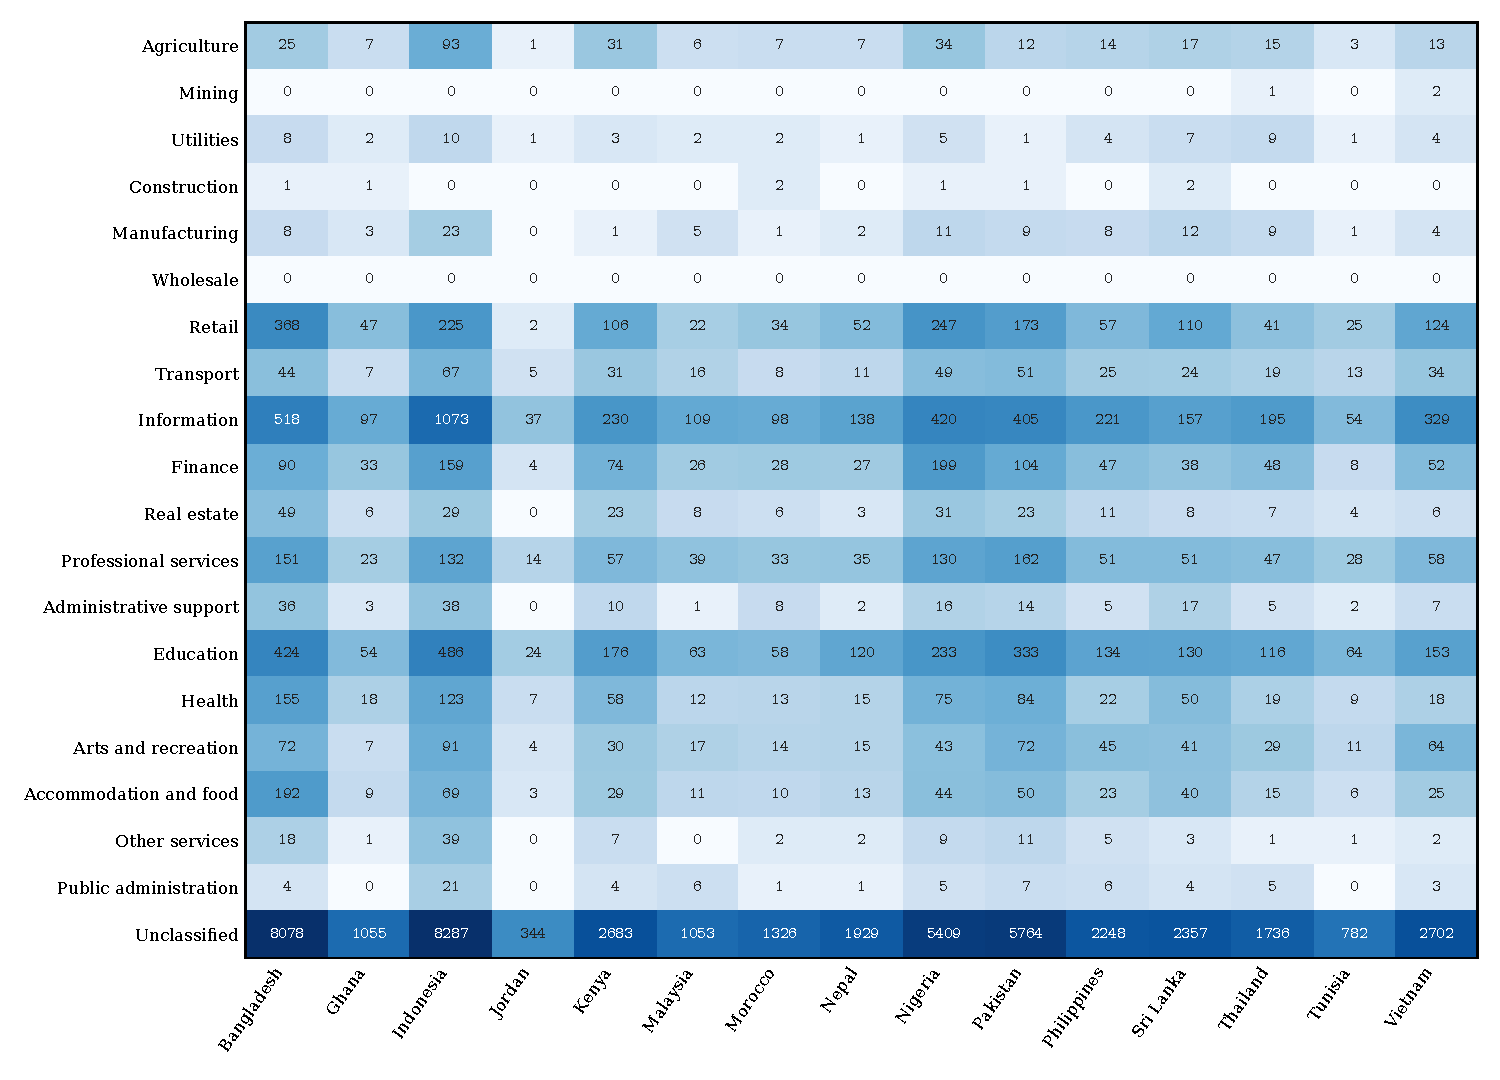
\includegraphics[width=\textwidth]{fig_evidence_country_domain_support.pdf}

\fignote{Numbers are fixed cohort sizes. Colour represents $\log_{10}(1+N)$ for readability. All 59,158 eligible users are assigned exactly once, including the unclassified group. The existing estimation screen requires at least 30 Bangladesh users and five donor countries with at least 30 users each; these descriptive figures apply no such deletion.}

\end{figure}\clearpage

\begin{figure}[p]\centering

\caption{Daily public activity in Bangladesh and every donor country}

\label{fig:country_national}

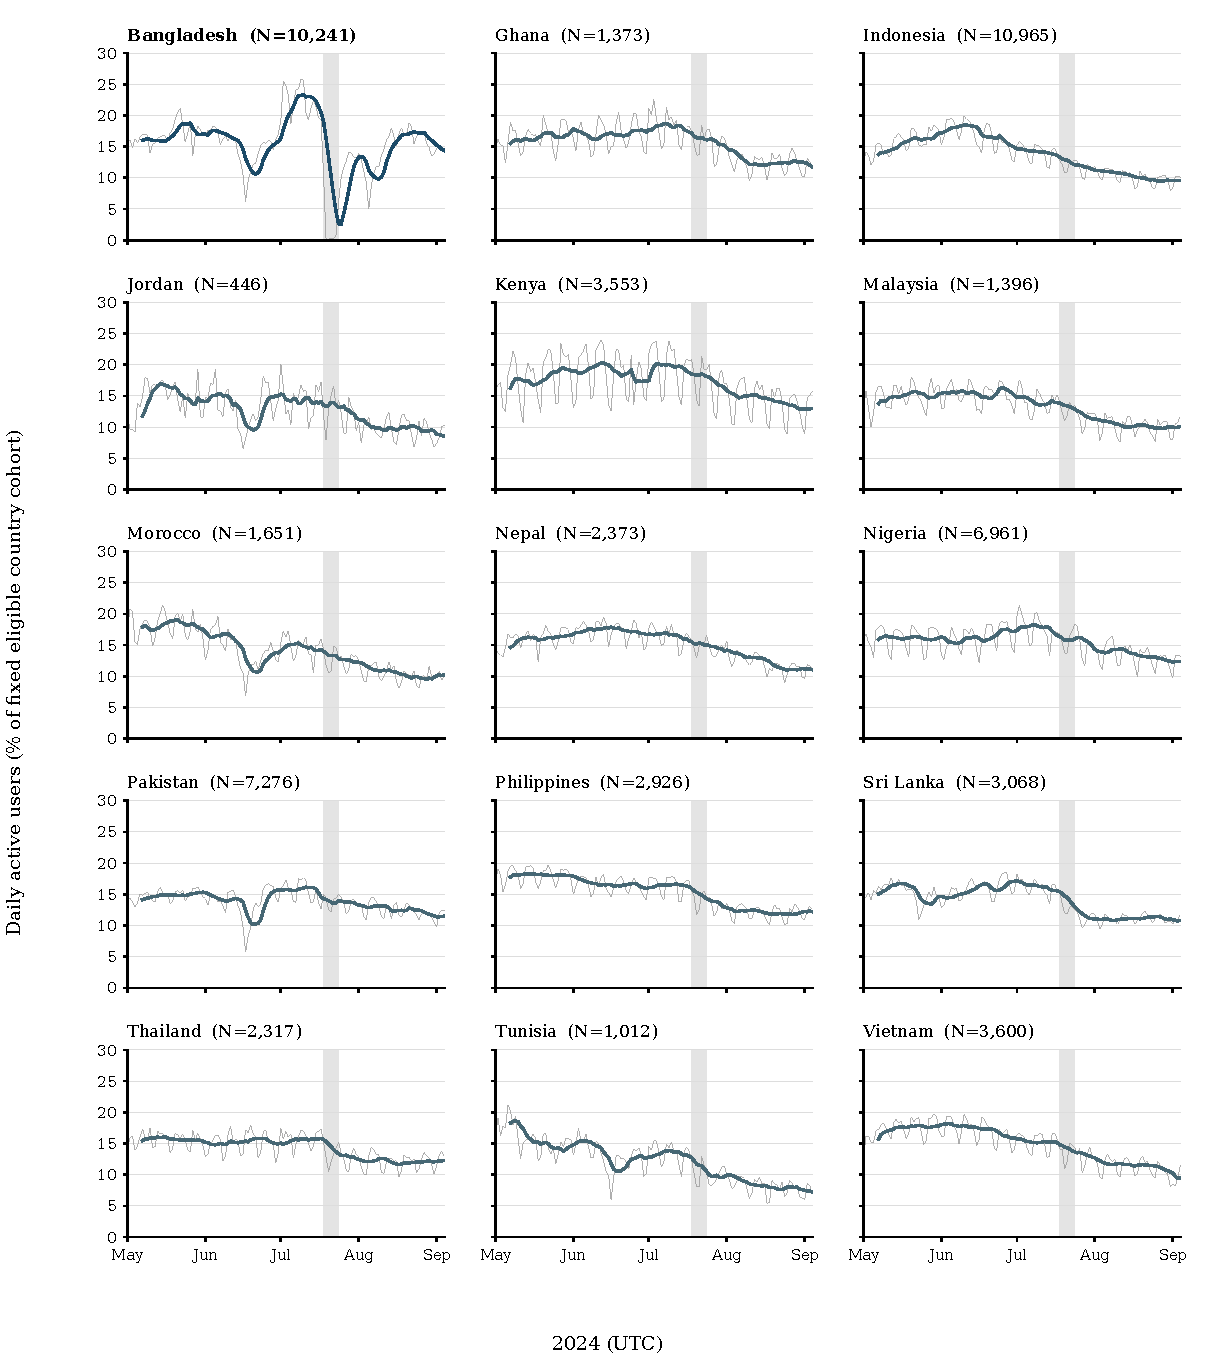
\includegraphics[width=\textwidth,height=.81\textheight,keepaspectratio]{fig_evidence_country_national.pdf}

\fignote{Thin grey lines: daily rates; coloured lines: trailing seven-day means, shown only after seven observations. Grey shading: July 18--23. All days and rates use UTC and the original country denominators. The smoothing is descriptive and is not used to re-estimate the primary model.}

\end{figure}\clearpage

\begin{figure}[p]\centering

\caption{Country-by-country public activity: Agriculture}

\label{fig:atlas_11}

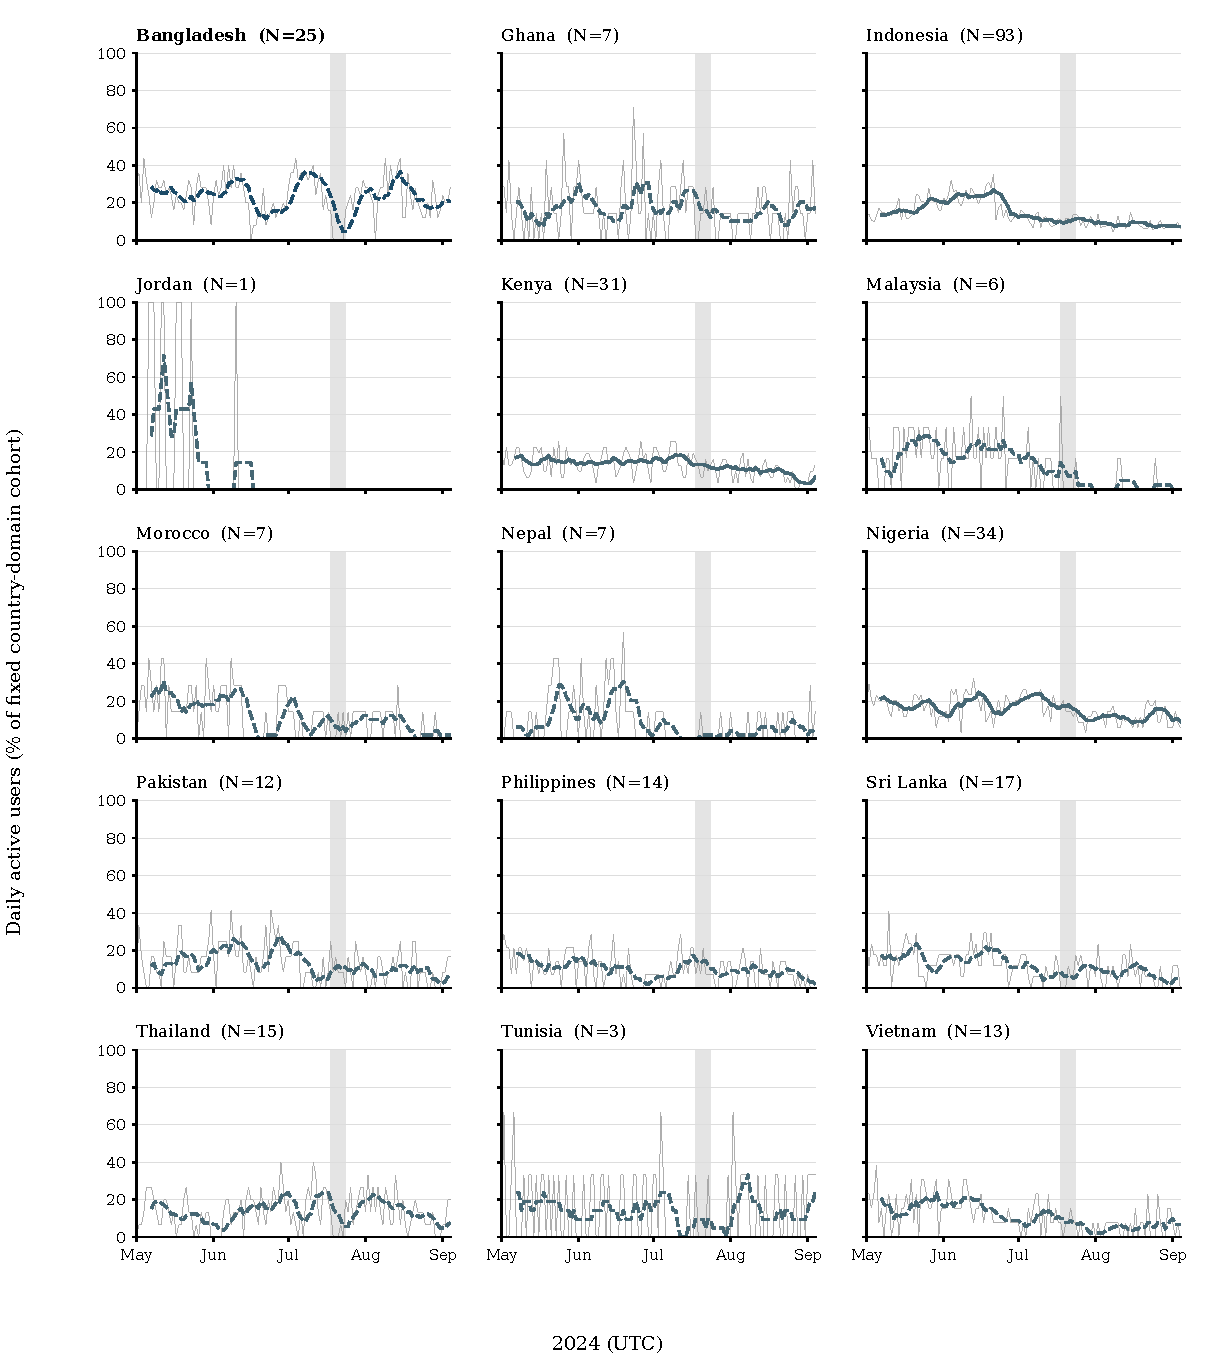
\includegraphics[page=1,width=\textwidth,height=.81\textheight,keepaspectratio]{fig_evidence_country_sectors.pdf}

\fignote{Fixed historical-README cohort, confidence threshold 0.80. Thin grey: daily rates; coloured: trailing seven-day mean. Dashed means indicate fewer than 30 users; empty cells have no assigned users. Scales are common across countries on this page but may differ across domains. Grey shading: July 18--23. The outcome counts each assigned user's primary activity anywhere on GitHub, not only activity in the repository used for assignment.}

\end{figure}\clearpage

\begin{figure}[p]\centering

\caption{Country-by-country public activity: Mining}

\label{fig:atlas_21}

\includegraphics[page=2,width=\textwidth,height=.81\textheight,keepaspectratio]{fig_evidence_country_sectors.pdf}

\fignote{Fixed historical-README cohort, confidence threshold 0.80. Thin grey: daily rates; coloured: trailing seven-day mean. Dashed means indicate fewer than 30 users; empty cells have no assigned users. Scales are common across countries on this page but may differ across domains. Grey shading: July 18--23. The outcome counts each assigned user's primary activity anywhere on GitHub, not only activity in the repository used for assignment.}

\end{figure}\clearpage

\begin{figure}[p]\centering

\caption{Country-by-country public activity: Utilities}

\label{fig:atlas_22}

\includegraphics[page=3,width=\textwidth,height=.81\textheight,keepaspectratio]{fig_evidence_country_sectors.pdf}

\fignote{Fixed historical-README cohort, confidence threshold 0.80. Thin grey: daily rates; coloured: trailing seven-day mean. Dashed means indicate fewer than 30 users; empty cells have no assigned users. Scales are common across countries on this page but may differ across domains. Grey shading: July 18--23. The outcome counts each assigned user's primary activity anywhere on GitHub, not only activity in the repository used for assignment.}

\end{figure}\clearpage

\begin{figure}[p]\centering

\caption{Country-by-country public activity: Construction}

\label{fig:atlas_23}

\includegraphics[page=4,width=\textwidth,height=.81\textheight,keepaspectratio]{fig_evidence_country_sectors.pdf}

\fignote{Fixed historical-README cohort, confidence threshold 0.80. Thin grey: daily rates; coloured: trailing seven-day mean. Dashed means indicate fewer than 30 users; empty cells have no assigned users. Scales are common across countries on this page but may differ across domains. Grey shading: July 18--23. The outcome counts each assigned user's primary activity anywhere on GitHub, not only activity in the repository used for assignment.}

\end{figure}\clearpage

\begin{figure}[p]\centering

\caption{Country-by-country public activity: Manufacturing}

\label{fig:atlas_31-33}

\includegraphics[page=5,width=\textwidth,height=.81\textheight,keepaspectratio]{fig_evidence_country_sectors.pdf}

\fignote{Fixed historical-README cohort, confidence threshold 0.80. Thin grey: daily rates; coloured: trailing seven-day mean. Dashed means indicate fewer than 30 users; empty cells have no assigned users. Scales are common across countries on this page but may differ across domains. Grey shading: July 18--23. The outcome counts each assigned user's primary activity anywhere on GitHub, not only activity in the repository used for assignment.}

\end{figure}\clearpage

\begin{figure}[p]\centering

\caption{Country-by-country public activity: Wholesale}

\label{fig:atlas_42}

\includegraphics[page=6,width=\textwidth,height=.81\textheight,keepaspectratio]{fig_evidence_country_sectors.pdf}

\fignote{Fixed historical-README cohort, confidence threshold 0.80. Thin grey: daily rates; coloured: trailing seven-day mean. Dashed means indicate fewer than 30 users; empty cells have no assigned users. Scales are common across countries on this page but may differ across domains. Grey shading: July 18--23. The outcome counts each assigned user's primary activity anywhere on GitHub, not only activity in the repository used for assignment.}

\end{figure}\clearpage

\begin{figure}[p]\centering

\caption{Country-by-country public activity: Retail}

\label{fig:atlas_44-45}

\includegraphics[page=7,width=\textwidth,height=.81\textheight,keepaspectratio]{fig_evidence_country_sectors.pdf}

\fignote{Fixed historical-README cohort, confidence threshold 0.80. Thin grey: daily rates; coloured: trailing seven-day mean. Dashed means indicate fewer than 30 users; empty cells have no assigned users. Scales are common across countries on this page but may differ across domains. Grey shading: July 18--23. The outcome counts each assigned user's primary activity anywhere on GitHub, not only activity in the repository used for assignment.}

\end{figure}\clearpage

\begin{figure}[p]\centering

\caption{Country-by-country public activity: Transport}

\label{fig:atlas_48-49}

\includegraphics[page=8,width=\textwidth,height=.81\textheight,keepaspectratio]{fig_evidence_country_sectors.pdf}

\fignote{Fixed historical-README cohort, confidence threshold 0.80. Thin grey: daily rates; coloured: trailing seven-day mean. Dashed means indicate fewer than 30 users; empty cells have no assigned users. Scales are common across countries on this page but may differ across domains. Grey shading: July 18--23. The outcome counts each assigned user's primary activity anywhere on GitHub, not only activity in the repository used for assignment.}

\end{figure}\clearpage

\begin{figure}[p]\centering

\caption{Country-by-country public activity: Information}

\label{fig:atlas_51}

\includegraphics[page=9,width=\textwidth,height=.81\textheight,keepaspectratio]{fig_evidence_country_sectors.pdf}

\fignote{Fixed historical-README cohort, confidence threshold 0.80. Thin grey: daily rates; coloured: trailing seven-day mean. Dashed means indicate fewer than 30 users; empty cells have no assigned users. Scales are common across countries on this page but may differ across domains. Grey shading: July 18--23. The outcome counts each assigned user's primary activity anywhere on GitHub, not only activity in the repository used for assignment.}

\end{figure}\clearpage

\begin{figure}[p]\centering

\caption{Country-by-country public activity: Finance}

\label{fig:atlas_52}

\includegraphics[page=10,width=\textwidth,height=.81\textheight,keepaspectratio]{fig_evidence_country_sectors.pdf}

\fignote{Fixed historical-README cohort, confidence threshold 0.80. Thin grey: daily rates; coloured: trailing seven-day mean. Dashed means indicate fewer than 30 users; empty cells have no assigned users. Scales are common across countries on this page but may differ across domains. Grey shading: July 18--23. The outcome counts each assigned user's primary activity anywhere on GitHub, not only activity in the repository used for assignment.}

\end{figure}\clearpage

\begin{figure}[p]\centering

\caption{Country-by-country public activity: Real estate}

\label{fig:atlas_53}

\includegraphics[page=11,width=\textwidth,height=.81\textheight,keepaspectratio]{fig_evidence_country_sectors.pdf}

\fignote{Fixed historical-README cohort, confidence threshold 0.80. Thin grey: daily rates; coloured: trailing seven-day mean. Dashed means indicate fewer than 30 users; empty cells have no assigned users. Scales are common across countries on this page but may differ across domains. Grey shading: July 18--23. The outcome counts each assigned user's primary activity anywhere on GitHub, not only activity in the repository used for assignment.}

\end{figure}\clearpage

\begin{figure}[p]\centering

\caption{Country-by-country public activity: Professional services}

\label{fig:atlas_54}

\includegraphics[page=12,width=\textwidth,height=.81\textheight,keepaspectratio]{fig_evidence_country_sectors.pdf}

\fignote{Fixed historical-README cohort, confidence threshold 0.80. Thin grey: daily rates; coloured: trailing seven-day mean. Dashed means indicate fewer than 30 users; empty cells have no assigned users. Scales are common across countries on this page but may differ across domains. Grey shading: July 18--23. The outcome counts each assigned user's primary activity anywhere on GitHub, not only activity in the repository used for assignment.}

\end{figure}\clearpage

\begin{figure}[p]\centering

\caption{Country-by-country public activity: Administrative support}

\label{fig:atlas_56}

\includegraphics[page=13,width=\textwidth,height=.81\textheight,keepaspectratio]{fig_evidence_country_sectors.pdf}

\fignote{Fixed historical-README cohort, confidence threshold 0.80. Thin grey: daily rates; coloured: trailing seven-day mean. Dashed means indicate fewer than 30 users; empty cells have no assigned users. Scales are common across countries on this page but may differ across domains. Grey shading: July 18--23. The outcome counts each assigned user's primary activity anywhere on GitHub, not only activity in the repository used for assignment.}

\end{figure}\clearpage

\begin{figure}[p]\centering

\caption{Country-by-country public activity: Education}

\label{fig:atlas_61}

\includegraphics[page=14,width=\textwidth,height=.81\textheight,keepaspectratio]{fig_evidence_country_sectors.pdf}

\fignote{Fixed historical-README cohort, confidence threshold 0.80. Thin grey: daily rates; coloured: trailing seven-day mean. Dashed means indicate fewer than 30 users; empty cells have no assigned users. Scales are common across countries on this page but may differ across domains. Grey shading: July 18--23. The outcome counts each assigned user's primary activity anywhere on GitHub, not only activity in the repository used for assignment.}

\end{figure}\clearpage

\begin{figure}[p]\centering

\caption{Country-by-country public activity: Health}

\label{fig:atlas_62}

\includegraphics[page=15,width=\textwidth,height=.81\textheight,keepaspectratio]{fig_evidence_country_sectors.pdf}

\fignote{Fixed historical-README cohort, confidence threshold 0.80. Thin grey: daily rates; coloured: trailing seven-day mean. Dashed means indicate fewer than 30 users; empty cells have no assigned users. Scales are common across countries on this page but may differ across domains. Grey shading: July 18--23. The outcome counts each assigned user's primary activity anywhere on GitHub, not only activity in the repository used for assignment.}

\end{figure}\clearpage

\begin{figure}[p]\centering

\caption{Country-by-country public activity: Arts and recreation}

\label{fig:atlas_71}

\includegraphics[page=16,width=\textwidth,height=.81\textheight,keepaspectratio]{fig_evidence_country_sectors.pdf}

\fignote{Fixed historical-README cohort, confidence threshold 0.80. Thin grey: daily rates; coloured: trailing seven-day mean. Dashed means indicate fewer than 30 users; empty cells have no assigned users. Scales are common across countries on this page but may differ across domains. Grey shading: July 18--23. The outcome counts each assigned user's primary activity anywhere on GitHub, not only activity in the repository used for assignment.}

\end{figure}\clearpage

\begin{figure}[p]\centering

\caption{Country-by-country public activity: Accommodation and food}

\label{fig:atlas_72}

\includegraphics[page=17,width=\textwidth,height=.81\textheight,keepaspectratio]{fig_evidence_country_sectors.pdf}

\fignote{Fixed historical-README cohort, confidence threshold 0.80. Thin grey: daily rates; coloured: trailing seven-day mean. Dashed means indicate fewer than 30 users; empty cells have no assigned users. Scales are common across countries on this page but may differ across domains. Grey shading: July 18--23. The outcome counts each assigned user's primary activity anywhere on GitHub, not only activity in the repository used for assignment.}

\end{figure}\clearpage

\begin{figure}[p]\centering

\caption{Country-by-country public activity: Other services}

\label{fig:atlas_81}

\includegraphics[page=18,width=\textwidth,height=.81\textheight,keepaspectratio]{fig_evidence_country_sectors.pdf}

\fignote{Fixed historical-README cohort, confidence threshold 0.80. Thin grey: daily rates; coloured: trailing seven-day mean. Dashed means indicate fewer than 30 users; empty cells have no assigned users. Scales are common across countries on this page but may differ across domains. Grey shading: July 18--23. The outcome counts each assigned user's primary activity anywhere on GitHub, not only activity in the repository used for assignment.}

\end{figure}\clearpage

\begin{figure}[p]\centering

\caption{Country-by-country public activity: Public administration}

\label{fig:atlas_92}

\includegraphics[page=19,width=\textwidth,height=.81\textheight,keepaspectratio]{fig_evidence_country_sectors.pdf}

\fignote{Fixed historical-README cohort, confidence threshold 0.80. Thin grey: daily rates; coloured: trailing seven-day mean. Dashed means indicate fewer than 30 users; empty cells have no assigned users. Scales are common across countries on this page but may differ across domains. Grey shading: July 18--23. The outcome counts each assigned user's primary activity anywhere on GitHub, not only activity in the repository used for assignment.}

\end{figure}\clearpage

\begin{figure}[p]\centering

\caption{Country-by-country public activity: Unclassified}

\label{fig:atlas_Unclassified}

\includegraphics[page=20,width=\textwidth,height=.81\textheight,keepaspectratio]{fig_evidence_country_sectors.pdf}

\fignote{Fixed historical-README cohort, confidence threshold 0.80. Thin grey: daily rates; coloured: trailing seven-day mean. Dashed means indicate fewer than 30 users; empty cells have no assigned users. Scales are common across countries on this page but may differ across domains. Grey shading: July 18--23. The outcome counts each assigned user's primary activity anywhere on GitHub, not only activity in the repository used for assignment.}

\end{figure}\clearpage
